\chapter{Beispielkapitel}
Zu Beginn eines Kapitels kann eine kurze Zusammenfassung des
Inhalts des Kapitels stehen, die nicht mehr als zehn Zeilen
umfassen sollte. 

\section{Erster Abschnitt}
Jedes Kapitel wird in Abschnitte gegliedert, die wiederum
in Unterabschnitte aufgeteilt werden k\"onnnen. 

\subsection{Erster Unterabschnitt}
Hier folgt der erste Unterabschnitt.

\subsection{Zweiter Unterabschnitt}
Hier folgt der zweite Unterabschnitt.

\section{Verschiedene Formeldarstellungen}
Formeln k\"onnen im Flie\ss text enthalten sein beispielsweise
$a^2+b^2=c^2$ oder im {\em Display}-Format
\[
a^2 + b^2 = c^2.
\]

\section{Umgebungen}
Umgebungen f\"ur S\"atze, Beispiele, Bemerkungen usw. verleihen
der Arbeit Struktur. 

\begin{satz}[Satz des Pythagoras]\label{satz:pythagoras}
In jedem rechtwinkligen Dreieck gilt $a^2+b^2=c^2$. 
\end{satz}

\begin{proof}[Beweis]
...
\end{proof}

\section{Einbinden von Grafiken und Programmcode}

\subsection{Grafiken} 
Eine Skizze der Konstruktion ist in Abbildung~\ref{fig:skizze}
dargestellt. 

\begin{figure}
\begin{center}
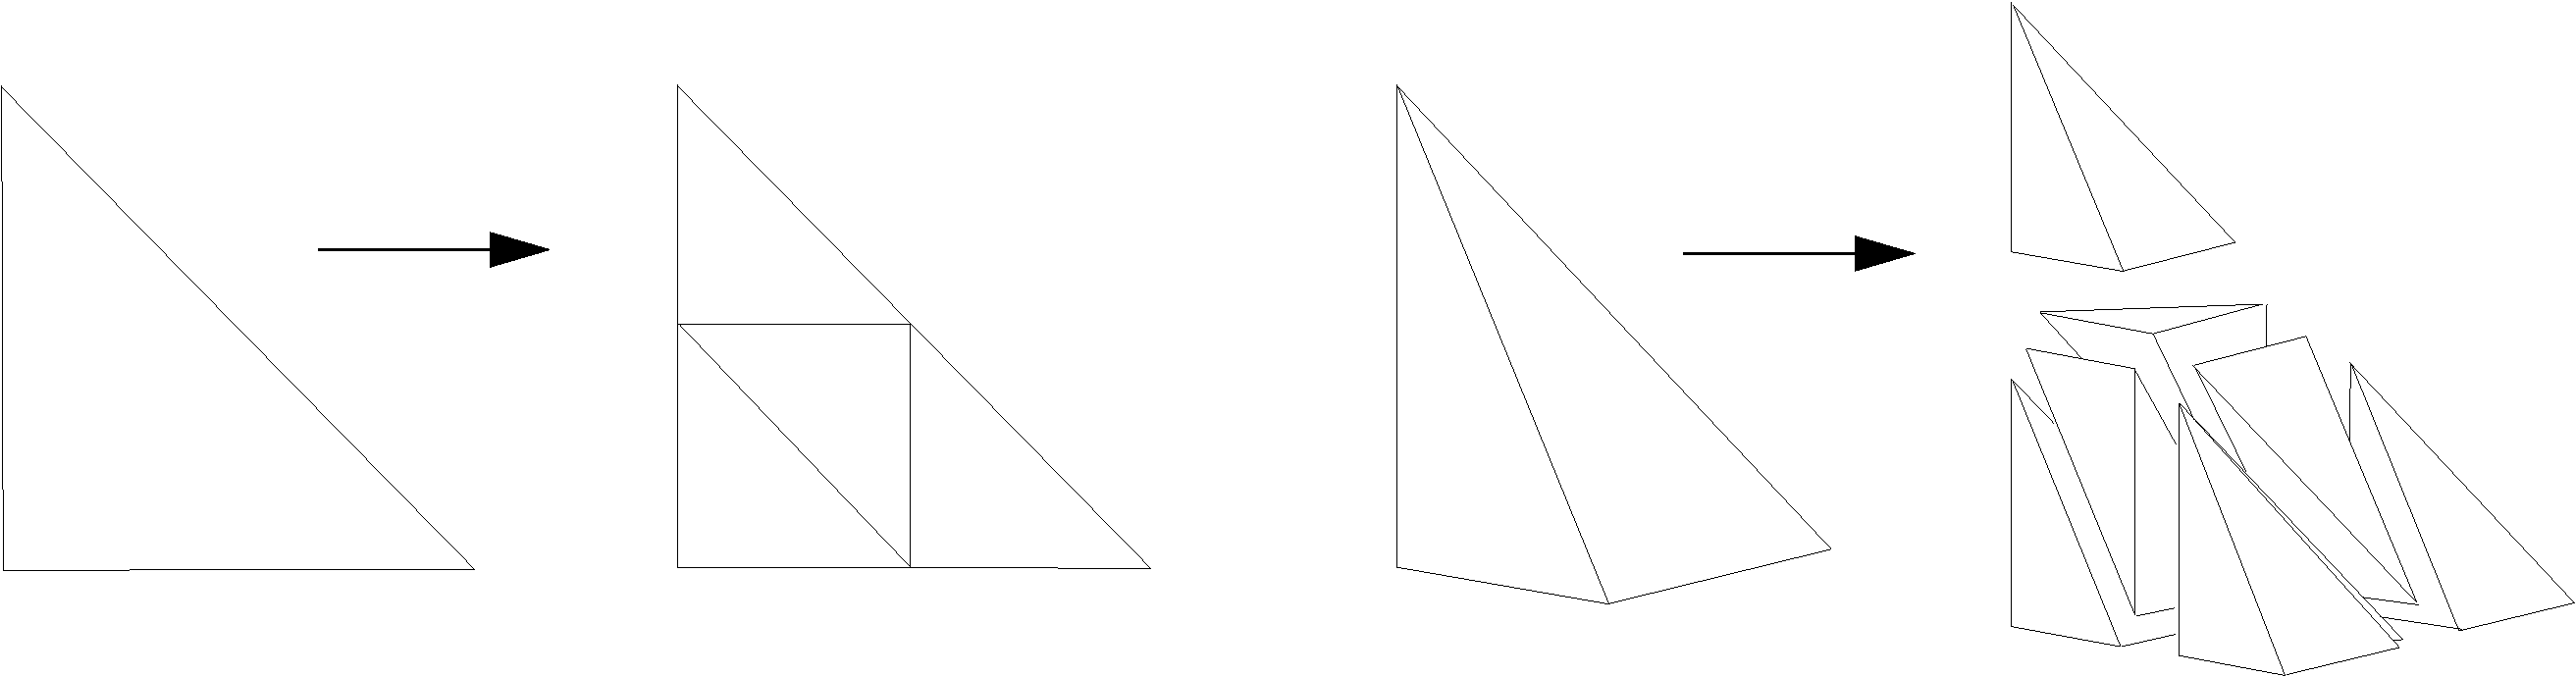
\includegraphics[width=8cm]{pics/beispiel_skizze.pdf}
\end{center}
\caption{\label{fig:skizze} Uniforme Verfeinerung eines
Dreiecks und eines Tetraeders}
\end{figure}

\subsection{Programmcode}
In Abbildung~\ref{fig:matlab_code} ist eine Realisierung in 
\matlab\ gezeigt. 

\begin{figure}
\lstinputlisting{codes/matlab_beispiel.m}
\caption{\label{fig:matlab_code} \matlab-Implementation der
Berechnung der Minoren einer Liste von Matrizen}
\end{figure}

\section{Zitieren}
In~\cite[Theorem~9.99]{Evan10-book} wird gezeigt, dass
Lipschitz-stetige Funktionen schwach differenzierbar sind. 
Die Arbeit~\cite{Bart13-pre} ist
mit der Approximation ratenunabh\"angiger Evolutionsprobleme
befasst.  